\newpage

\section{Modelo de información: Consulta de Profesores & Horarios}

\subsection{Descripción general}

En la figura~\ref{fig:modeloinfoprofe} se muestra la estructura de información que manejará el sistema para registrar la información de los datos personales, datos del domicilio, datos de contacto e información escolar del aspirante.

\begin{figure}[htbp!]
	\begin{center}
		\fbox{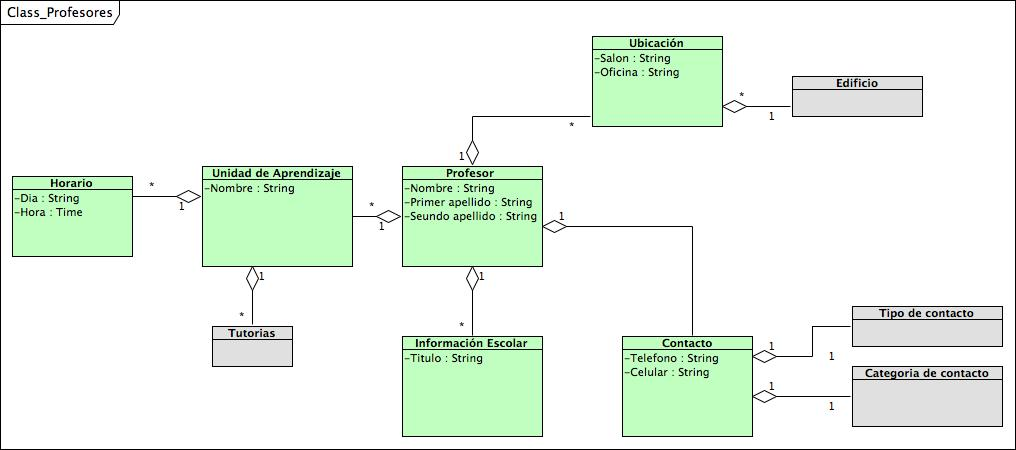
\includegraphics[width=1\textwidth]{images/Modelo_info_Profesores.jpg}}
		\caption{Modelo de información de consulta de profesores.}
		\label{fig:modeloinfoprofe}
	\end{center}
\end{figure}


%--------------------------------------------------------------------------------
\begin{BusinessEntity}{persona}{Persona}
	
	\Battr{nombre}{Nombre}{\tdFrase}{Denominación que se le da a una persona}{\requerido}{\longitudMinMax{1}{caracteres}{20}{caracteres}}
	
	\Battr{primerApellido}{Primer apellido}{\tdPalabra}{Apellido paterno de una persona}{\requerido}{\longitudMinMax{1}{caracteres}{20}{caracteres}}
	
	\Battr{segundoApellido}{Segundo apellido}{\tdPalabra}{Apellido materno de una persona}{\opcional}{\longitudMinMax{1}{caracteres}{20}{caracteres}}
	
\end{BusinessEntity}

%--------------------------------------------------------------------------------
\begin{BusinessEntity}{Ubicacion}{Ubicación}
	
	\Battr{salon}{Salón}{\tdFrase}{Nombre que se le da a un determinado lugar}{\requerido}{\longitudMinMax{1}{caracteres}{4}{caracteres}}
	
	\Battr{oficina}{Oficina}{\tdFrase}{Nombre oficial de una escuela}{\requerido}{\longitudMinMax{1}{caracteres}{20}{caracteres}}
	
	
\end{BusinessEntity}

%--------------------------------------------------------------------------------
\begin{BusinessEntity}{InformacionEscolar}{Información Escolar}
	
	\Battr{titulo}{Título}{\tdCatalogo}{Se refiere al \cdtRef{gls:medioContacto}{tipo de contacto}}{\requerido}
	
\end{BusinessEntity}

%--------------------------------------------------------------------------------
\begin{BusinessEntity}{contacto}{Contacto}
	
	\Battr{telefono}{Teléfono}{\tdCatalogo}{Se refiere al \cdtRef{gls:medioContacto}{tipo de contacto}}{\opcional}{\longitudExacta{8}{dígitos}}
	
	\Battr{celular}{Celular}{\tdCatalogo}{Se refiere al \cdtRef{gls:medioContacto}{tipo de contacto}}{\opcional}{\longitudExacta{10}{dígitos}}
	
	
\end{BusinessEntity}

%--------------------------------------------------------------------------------
\begin{BusinessEntity}{unidadaprendizaje}{Unidad de Aprendizaje}
	
	\Battr{nombre}{Nombre}{\tdFrase}{Denominación que se le da a una persona}{\requerido}{\longitudMinMax{1}{caracteres}{50}{caracteres}}
	\Battr{nivel}{Nivel}{\tdPalabra}{Denominación que se le da a un nivel de la Escuela Superior de Cómputo.}{\requerido}{\longitudExacta{1s}{dígitos}}
	
\end{BusinessEntity}


%--------------------------------------------------------------------------------
\begin{BusinessEntity}{horario}{Horario}
	
	\Battr{dia}{Día}{\tdFecha}{Se refiere al día de la semana de una clase}{\requerido}
	\Battr{hora}{Hora}{\tdHora}{Se refiere a al hora en la que se imparte una unidad de aprendizaje.}{\requerido}
	
\end{BusinessEntity}